% -- makrot ja muut alkutavarat kuuluisivat ehk�p� loogisemmin dokumentti.tex -tiedostoon, mutta kun niit� kuitenkin pit�� jatkuvasti muokkailla, ei se olisi ollenkaan k�tev��

% est�mme ihme "underfull \hbox (badness 10000)" -varoitukset (ei hajua mist� tulevat)
\hbadness=10000

% makrot dokumentoinnin generoimiseksi
% Macros for generating Test Cases

% MACROS FOR TEST CASE

\newcounter{successTest}
\newcounter{overallTest}
\newcommand{\getClass}[0]{}
\newcommand{\beginTestedClass}[1] {
	\subsection{#1}
	\renewcommand{\getClass}[0]{#1}
	\begin{enumerate}
}
\newcommand{\beginCase}[1] {
	\item #1
}
\newcommand{\beginConditions}[0] {
	Conditions:
	\begin{itemize}
}
\newcommand{\condition}[1] {
	\item #1
}
\newcommand{\testParam}[1] {
	\\
	\textbf{Tested parameter}: #1
}
\newcommand{\testResultTrue}[0] {
	\\
	\textbf{Result}: success
	\stepcounter{overallTest}
	\stepcounter{successTest}
}
\newcommand{\testResultFalse}[0] {
	\\
	\textbf{Result}: failed
	\stepcounter{overallTest}
}
\newcommand{\closeConditions}[0] {
	\end{itemize}
}
\newcommand{\closeTestedClass}[0] {
	\end{enumerate}
	\textbf{Test results for \getClass   \arabic{successTest}/\arabic{overallTest}}
	\setcounter{overallTest}{0}
	\setcounter{successTest}{0}
}

% MACROS FOR GETTING RESULTS


% esimerkkirakenne mukaillen kopioitu ekasta l�yt�m�st�ni esimerkist� -> http://www.cs.helsinki.fi/group/assari/

\section{Introduction}

\subsection{Meaning and structure of the document}
\subsection{Glossary}


\section{Overview of the system}

% kuvan lis�ys ja siihen viittaus estetyll� rivinvaihdolla
\begin{figure}
\begin{center}
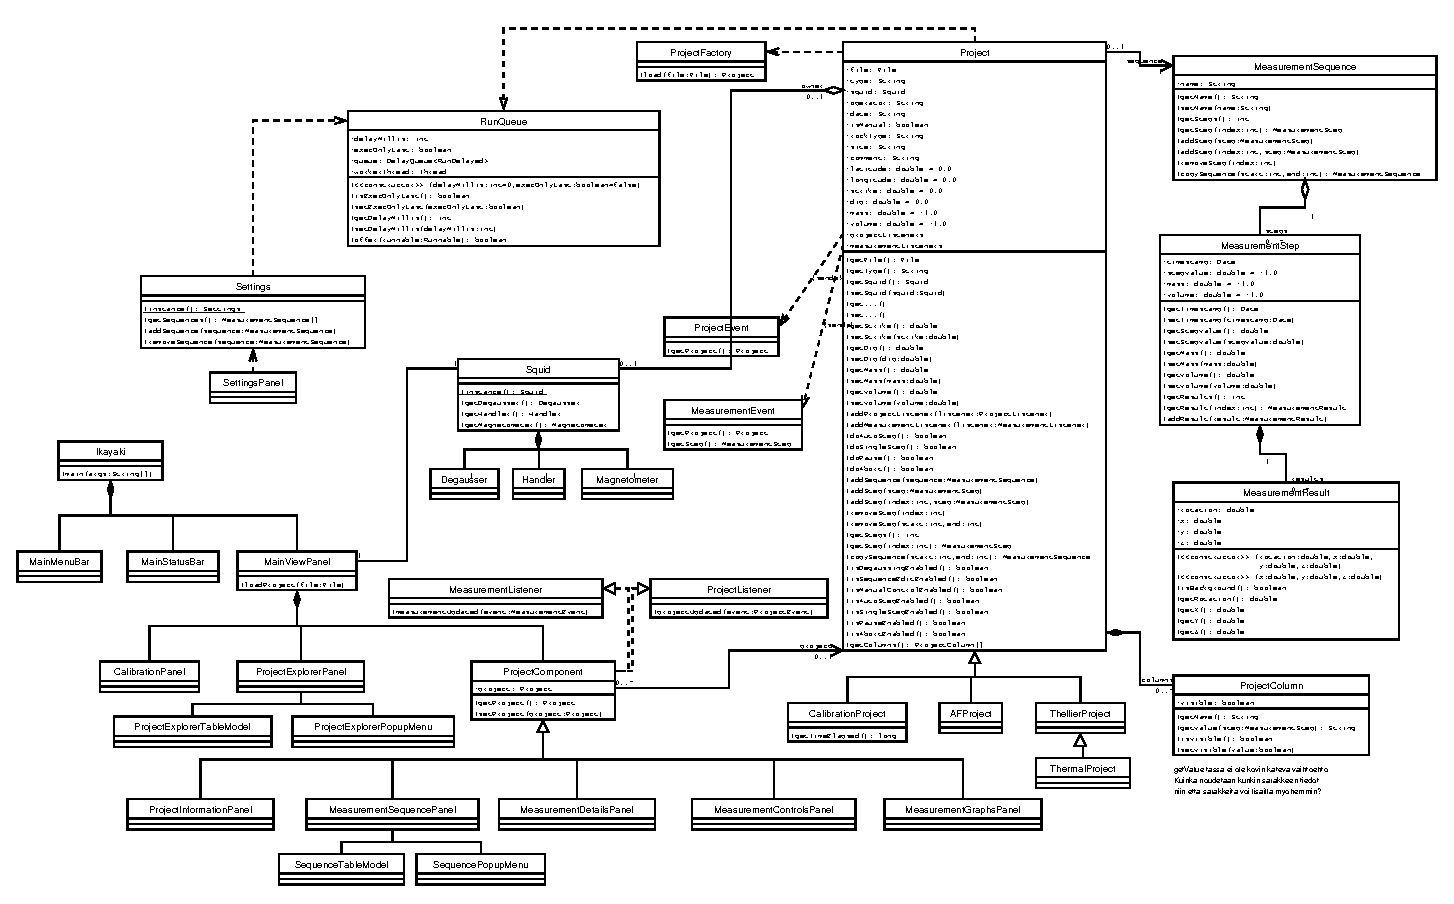
\includegraphics[angle=90,width=14cm]{class-diagram.eps}
\caption{Squid class diagram}
\label{fig:classdiagram}
\end{center}
\end{figure}

See Figure~\ref{fig:classdiagram}.


\section{Architecture description}


\section{Project Explorer}

\subsection{ProjectExplorerPanel}

Created by: MainViewPanel \\
Uses: ProjectExplorerTableModel, ProjectExplorerPopupMenu

Creates a history/autocomplete field (browserField) for choosing the project directory, a listing of project files in that directory (explorerTable) and in that listing a line for creating new project, which has a textbox for project name, an AF/TH ComboBox and a "Create new" button for actuating the creation. Also has a right-click popup menu for exporting project files.

Events:

- On browserField change: send browserField's text to RunQueue (singleton?) which schedules disk access and autocomplete. (This could be in a separate BrowserFieldComponent class...) \\
- On explorerTable mouse right-click: create a ProjectExplorerPopupMenu for right-clicked project file (this could be in ProjectExplorerTableModel class). \\
- On createNewProject mouseclick: create a new project, set it active and tell ProjectExplorerTableMode to update itself. \\
- On browseButton mouseclick: open a FileChooser dialog for choosing the directory.

Fields: (not all necessarily needed, most are also self explanatory) \\
- BrowserFieldComponent browserField (need a separate class for this?) \\
- ProjectExplorerTableModel explorerTable \\
- JButton createNewProject \\
- JButton browseButton \\
- JTextField newProject \\
- JComboBox newProjectType

Constructors:

- ProjectExplorerPanel()

Creates its components, places them and sets the last project folder as current project folder.

Methods:

- public void createNewProject()

Creates a new project, sets it active, sends it to MainViewPanel, tells explorerTable to reset newProject and newProjectType fields.

- public void doBrowse()

Creates a FileChooser dialog and tells explorerTable and browserField to change to directory returned by it.

\subsection{ProjectExplorerTableModel}

Created by: ProjectExplorerPanel

Creates a list of project files in directory and handles changes the selected project and executing export choice.

Events:

- On newDirectoryEvent: updates list of project files on JTable \\
- On selectTable MouseEvent: sets new Project active

Fields: \\
- JTable projectFiles

Constructors:

- ProjectExplorerTableModel()

Creates projectFiles and gets its content from default directory

- ProjectExplorerTableModel(String directory)

Creates projectFiles and gets its content from given directory

Methods:

- public void loadDirectory(String directory)

Update list to show given directory.

- public void loadProject()

gets selected line from list and send it to MainViewPanel.

\subsection{ProjectExplorerPopupMenu}

Created by: ProjectExplorerPanel

Shows choices to export: AF, Thellier, Thermal and executes selected

Events:

- On selectItem mouseEvent: tells selected Project to create selected file from it's self

Fields:

Constructors:

- ProjectExplorerTableModel()

Creates itself

Methods:

- public void export(int type)

Tells current project to export itself to selected type.


\section{Some other specific part (subsystem) to this system...}

\section{Package structure}

\section{Bibliography}
